\section{Questionnaire result and discussion}




The questionnaire remained open for a week, during which time it garnered responses from a total of 136 anonymous participants.
Since we shared the link out to friends and family, we are expecting the age distribution of the participants to be mainly around 18 to 25, with some participants reaching age 50 and above.
From our friend groups and family members, we assume all the participants to the questionnaire has basic knowledge to technology, such as navigate through websites or using social media.

\begin{figure}[ht]
  \centering
  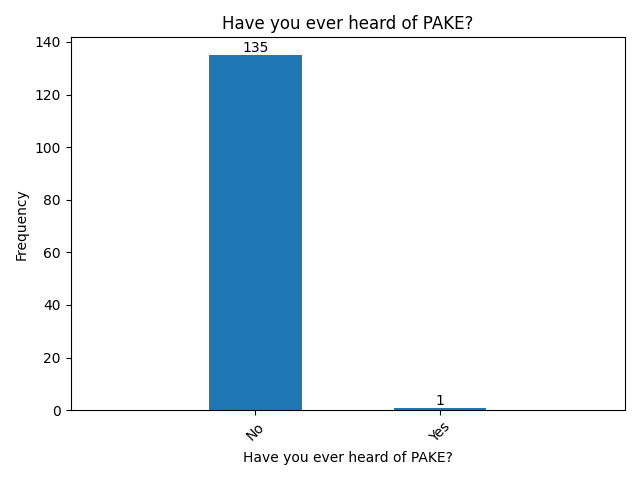
\includegraphics[width=0.4\textwidth]{./images/know_pake.png}
  \caption{TODO: change caption}
  \label{fig:know_pake}
\end{figure}

\subsection{Knowledge about PAKE}
We asked the participants whether they have heard about PAKE protocols or not.
Initially, we did not expect any participants to know anything about PAKE, speaking from our experience that none of us knew PAKE until we start working on the project.
But surprisingly, one participant out of 136 actually knew about PAKE protocols with prior knowledge, as shown in ~\figref{fig:know_pake}.
They highlighted that "PAKE protocols use zero-knowledge proofs to authenticate without transmitting passwords. Good for security," which is the goal PAKE is aiming to achieve.





\begin{figure}[ht]
  \centering
  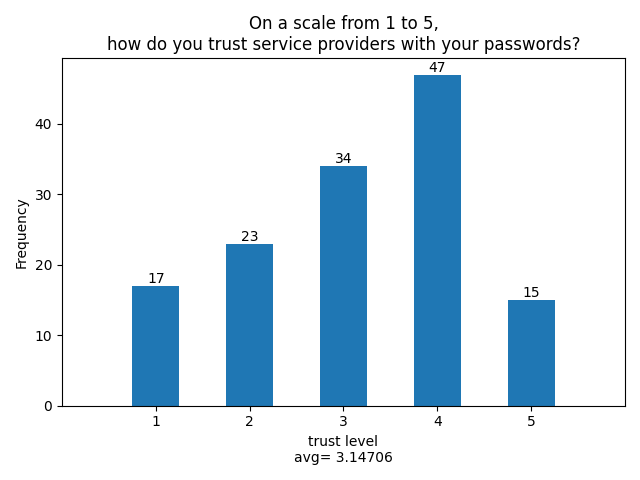
\includegraphics[width=0.4\textwidth]{./images/service_provider_trust.png}
  \caption{TODO: change caption}
  \label{fig:trust}
\end{figure}


\subsection{Trust to Password over TLS and service providers}
We are also curious how users trust service providers with their password.
We informed the participants that Password over TLS implementation requires storing encrypted password in the service providers' databases, and wanted to collect some feedback for this implementation.
Most answers surrounded the idea of data breach and leaks, which is one way an adversary gain control of a user's account.
One participant mentioned that "widely-used authentication methods, once subject to a data breach, are completely vulnerable: all users' data can be extracted, as user passwords are entirely stored on the server side databases."
While this is not entirely correct, storing password in server's database can add additional risks to lose all other personal data stored with the service provider.

Another participant mentioned password reusing, which he said most people would not bother to remember multiple passwords to different services, which can put all the services that use same password in danger if one of them is breached.
He also said in order to prevent the incident from happening, users often use password managers or notebook applications to keep track their passwords, but the additional use of programs brings another vulnerability to the potential leak of passwords.






\begin{figure}[ht]
  \centering
  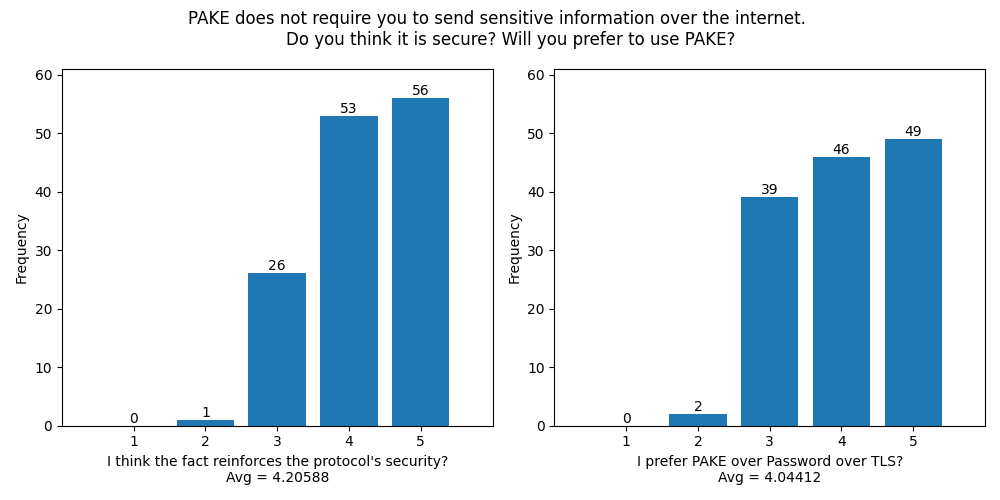
\includegraphics[width=0.4\textwidth]{./images/secure_preference.png}
  \label{fig:}
  \caption{TODO: change caption}
\end{figure}

\subsection{Preference between PAKE and Password over TLS}








\begin{figure}[ht]
  \centering
  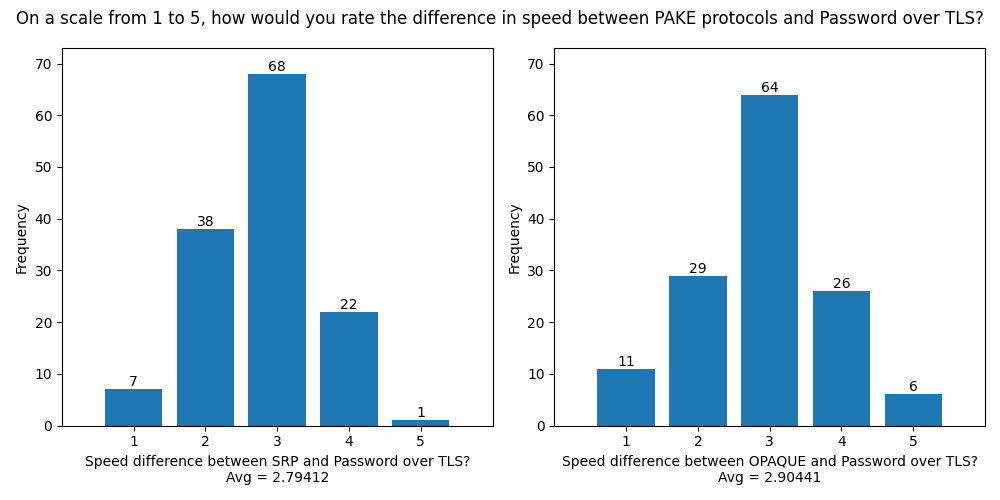
\includegraphics[width=0.4\textwidth]{./images/ux_compare.png}
  \label{fig:}
  \caption{TODO: change caption}
\end{figure}


\subsection{User experience analysis}